\section{Mikroprogrammierung}
		Durch Mikroprogrammierung muss nicht zwangsläufig jeder Befehl fest verdrahtet sein, er kann auch emuliert werden. Besonders bei sehr großen Befehlssätzen (CISC(Complex Instruction Set Computer)) \newline \newline
		\textbf{Mikroprogrammierung} bedeutet, komplexe \textbf{Maschinenbefehle} zur Laufzeit in der CPU durch eine Reihe an noch kleineren, einfacheren Befehlen zu emulieren. \textbf{Assembler-Programme} sind demnach \textbf{Makroprogramme}
	\subsection{Aufbau}
		Ein Mirko-Programm besteht aus aus 4 Kernbestandteilen:
		\begin{itemize}
	  		\item Steuerleitungen
	  		\item ALU (Arithmetisch-logische Einheit)
	  		\item Zwischenregister
	  		\item Tri-State (Schalter zum Öffnen und Schließen der Datenleitungen)
		\end{itemize}
	\subsection{Horizontsal vs. vertikal}
		\subsubsection{Horizontal}
			Für jede Steuerleitung wird ein Bit im Mikrobefehl verwendet. Vorteil, keine Dekodierung. Nachteil, Speicherverschwednung
		\subsubsection{Vertikal}
			Steuerleitungen werden gruppiert, was zu kürzeren Mikrobefehlen führt. Vorteil, speichereffizient. Nachteil, zur Laufzeit muss der komprimierte Befehl wieder in Leitungssignale umgewandelt werden
	\subsection{Beispiel}
		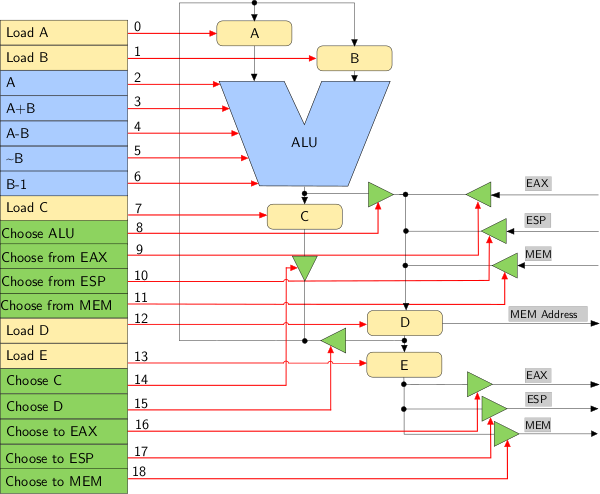
\includegraphics[scale=0.75]{mikroprogrammwerk.png}
		\begin{center}
			\begin{tabular} {|c|c|}
			\hline
			Zeile & Instruktion \\
			\hline
			0 & ESP $\rarr$ B \\
			\hline
			1 & B-1$\rarr$C \\
			\hline
			2 & C$\rarr$B \\
			\hline
			3 & B-1$\rarr$D \\
			\hline
			4 & D$\rarr$ESP \\
			\hline
		\end{tabular}	
		\end{center}
		
				
	